%%================================================
%% Filename: main.tex
%% Encoding: UTF-8
%% Author: Yuan Xiaoshuai - yxshuai@gmail.com
%% Created: 2012-01-08 13:09
%% Last modified: 2020-04-05 21:01
%%================================================
\documentclass[master]{zzuthesis}
% \documentclass[%
%   bachelor|master|doctor% mandatory option
%   ]{zzuthesis}
% 自定义宏包
\usepackage{docutils}

% 图形文件路径
\graphicspath{{figures/}}

\begin{document}

% 封面、目录、符号对照表等
\frontmatter

%%================================================
%% Filename: cover.tex
%% Encoding: UTF-8
%% Author: Yuan Xiaoshuai - yxshuai@gmail.com
%% Created: 2012-01-14 13:44
%% Last modified: 2019-11-03 00:30
%%================================================
% 研究生论文:学校代码、学号或申请号、密级
\schoolcode{10459}
\id{202112332015511}
\secretlevel{}

% 论文题目
\ctitle{基于贝叶斯网络的IPv6地址生成模型}

% 研究生论文:
% 培养院系、学科门类、专业名称、专业学位名称(仅限于专业博士、硕士学位论文)、
% 导师姓名、完成时间
% 本科论文:
% 指导老师、职称、学生姓名、学号、专业、院(系)、完成时间
\cdepartment{网络空间安全学院}
\csubject{工\hspace{2em}学}
\cmajor{网络空间安全}
\cauthor{张\hspace{2em}全} 
\csupervisor{李润知}
\protitle{副教授}%
\stuno{202112332015511}%本科论文需要学号
% 时间自动生成
% \submitdate{}
% \cdate{\CJKdigits{\the\year}年\CJKnumber{\the\month}月}
% \cdate{2012年6月}

% 研究生论文:英文封面
\etitle{IPv6 address generation model based on Bayesian network} 
\emajor{Cyberspace security} 
\edepartment{School of Cyberspace security}
\eauthor{Zhang Quan} 
\esupervisor{Prof. Li Runzhi} 
% \edate{December, 2005}%英文日期自动生成
%封面
\begin{cabstract}

  为解决 IPv6 网络扫描问题,本文提出了一种基于信息熵, DBSCAN, 贝叶斯网络等算法的 IPv6 地址生成模型. 该模型通过学习 IPv6 地址空间结构特征生成 IPv6 地址, 有效提高了 IPv6 网络扫描的效率.

  本文的创新点主要有:

  \begin{itemize}
  \item 基于半字节的信息熵进行段划分;
  \item 基于 DBSCAN 进行段分类;
  \item 基于贝叶斯网络进行关联性分析.
  \end{itemize}

\end{cabstract}

\ckeywords{IPv6; 信息熵; DBSCAN; 贝叶斯网络}

\begin{eabstract}

  In order to solve the problem of IPv6 network scanning, this paper proposes an IPv6 address generation model based on information entropy, DBSCAN, Bayesian network and other algorithms. This model generates IPv6 addresses by learning the IPv6 address space structure, which effectively improves the efficiency of IPv6 network scanning.

  The main innovations of this article are:

  \begin{itemize}
  \item Segmentation based on nibble information entropy;
  \item Segment classification based on DBSCAN;
  \item Relevance analysis based on Bayesian network.
  \end{itemize}

\end{eabstract}

\ekeywords{IPv6; Information entropy; DBSCAN; Bayesian network}
%摘要
\makecover

\tableofcontents%目录

% \listoffigures%插图清单,本科论文重新定义为\relax
% \listoftables%表格清单,本科论文重新定义为\relax

% \makeatletter%符号对照表
%   \ifzzu@bachelor\else\include{data/denotation}\fi%本科论文不要求
% \makeatother

% 正文部分
\mainmatter
\chapter{引言}
\label{cha:introduction}

\section{研究背景}

IPv4 网络扫描是简单的. IPv4 $2^{32}$ 的地址空间对现代计算机而言并非庞大, 使用了无状态技术的网络扫描工具如 Zmap, masscan 等可以在几个小时内扫描整个 IPv4 网络. 狭小的地址空间也限制了 IPv4 地址的配置方式: 网络管理员们试图充分利用每一个公网地址, 即使使用 NAT 技术的私有地址, 狭小的主机号地址空间也多由手动分配或使用 DHCP 连续分配. 这些因素都使得网络扫描工具如 nmap 可以快速扫描一个网段.

但 IPv6 则不同. IPv6 有巨大的 $2^{128}$ 的地址空间, 甚至 ISP 默认提供 $2^{96}$ 的地址空间. 凭借于此, IPv6 地址配置策略也多种多样: 除了继承自 IPv4 的手动分配和 DHCP, 常见的地址配置方式还有 EUI-64 和随机地址. 除此之外, 新的更加复杂的地址配置方式也被不断提出. 如充分利用 IPv6 地址空间, DHCP 每次分配单向加密过的无规律可循的 IPv6 地址. 这些因素使得以往在 IPv4 网络中常用的扫描工具对 IPv6 网络不再有效. 因此, 我们期望找到一个新的方法来扫描 IPv6 网络.

\section{研究方法概述}

IPv6 网络扫描的难点在于其巨大的地址空间. 本文的主要工作是提出了一种 IPv6 地址生成模型, 该模型通过对一组 IPv6 地址的学习, 了解 IPv6 地址空间结构, 进而生成 IPv6 地址. 通过该模型, 我们可以缩小 IPv6 地址空间, 提高 IPv6 网络扫描的效率.

该模型主要基于以下三个技术:

\begin{itemize}
\item 信息熵分析: 本文使用 IPv6 地址 32 个半字节的信息熵来判断其变动率, 通过比较相邻半字节的信息熵来对 IPv6 地址进行分段, 当相邻的半字节信息熵相近时, 便将其合并为一个更大的段. 例如, 数据集中如果存在大量遵循 EUI-64 规范的 IPv6 地址会降低第 23-26 个半字节的信息熵, 从而使 23-26 个半字节被合并为一段.
\item DBSCAN: 本文使用的第二个技术是基于 DBSCAN 算法对数据集进行无监督机器学习, 对基于信息熵分析划分的每个段的值进行聚类.
\item 贝叶斯网络: 本文使用的第三个技术是基于贝叶斯网络对数据集进行统计建模, 以一种分层的方式自动确定段值集群中的条件概率. 通过机器学习的方式发现基于信息熵的特征揭示 IPv6 地址空间结构要优于研究人员视觉检查大量 IPv6 地址.
\end{itemize}

该模型以循序渐进的方式, 首先收集数据集, 通过信息熵分析分段, 通过 DBSCAN 对段值聚类, 最后建立贝叶斯网络模型.

当扫描一个 IPv6 网络时, 我们不必扫描其内所有地址, 而是扫描通过该模型生成的若干地址. 这种扫描的准确性受制于数据集对要扫描的网络的代表性.

\section{相关工作}

早在 2004 年, Strayer 等人~\cite{ref:strayer}~就将信息熵分析应用到 IPv6 地址中. 他们注意到, IPv6 地址每字节的信息熵要原低于 IPv4, 这很好理解: 在 IPv6 地址中, 信息不必像 IPv4 地址那样压缩到 4 字节中, 相反, 信息可以在 IPv6 地址中传播. 从那时其起, IPv6 地址隐私扩展的引入和普及改变了这种状况, 它为 IPv6 地址增加了随机值, 从而抬高了信息熵. 虽然随机值有较高的信息量, 但都是一些不相关的网络结构. Malone~\cite{ref:malone}~, Gont 和 Chown~\cite{ref:gont}~, Plonka 和 Berger~\cite{ref:plonka}~ 等人的工作都尝试识别 IPv6 地址中的伪随机数, 本文也是如此, 不同的是本文利用了信息熵.
\chapter{研究方法}
\label{cha:methods}

\section{数据集}

本研究使用的数据集为 \href{https://ipv6hitlist.github.io}{https://ipv6hitlist.github.io} 提供的约 4 亿个 IPv6 地址. 这些地址是为 IPv6 网络扫描相关研究而收集并不断更新的可响应的 IPv6 地址集.

\section{信息熵分析}

信息熵是一种对信息的不可预测性的度量. 其定义为:

$$H(x) = - \sum\limits_{i=1}^{k} P(x_i) \log P(x_i)$$

一般而言, 信息熵越大, X 值的分布就越无序. 当信息熵为 0 时, X 为定值.

信息熵揭示了 IPv6 地址中可变部分与相对不可变部分. 我们提出了一个简单的基于阈值的分割算法, 用于基于信息熵将 IPv6 地址中相邻的半字节合并为一个地址段: 将相邻的半字节划分为一个段, 当相邻半字节信息熵的差超过阈值时开始新的段划分.

图~\ref{fig:entropy}~绘制了样本集每半字节的信息熵. 通过比较相邻半字节的信息熵, 我们将 IPv6 地址划分为若干地址段. 该图用虚线划分地址段, 用大写字母标记. 对于该样本集, 我们将其划分为 A-N 14 个地址段.

\begin{figure}[htbp]
\centering
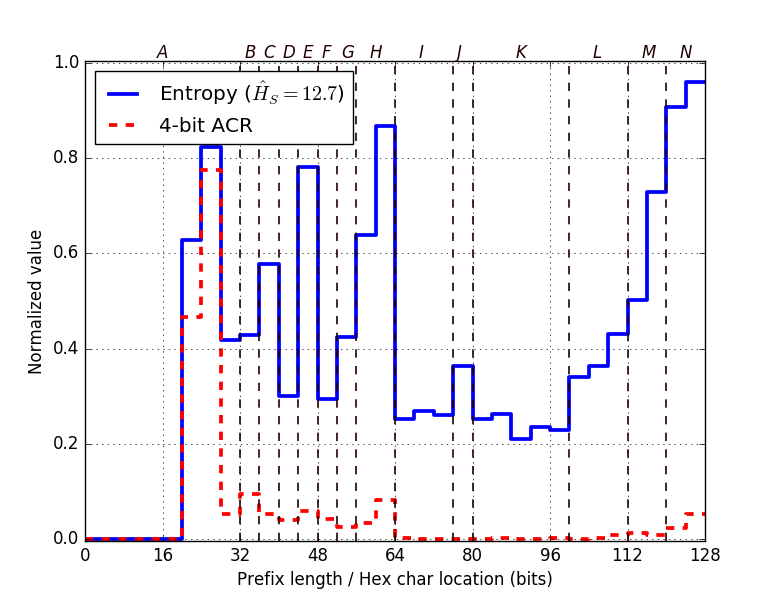
\includegraphics[width=0.5\textwidth]{entropy}
\caption{信息熵}
\label{fig:entropy}
\end{figure}

\section{DBSCAN}

在进一步分析中, 我们想要理解为什么一些值非随机的出现. 我们同时考虑值的频率和值本身, 提出了一个简单的基于阈值的聚类算法: 对每一个段, 首先找出那些出现频率超过阈值的值, 然后用基于密度的聚类算法 DBSCAN 对余下的值进行聚类.

图~\ref{fig:dbscan}~展示了部分样本集的聚类结果.

\begin{figure}[htbp]
\centering
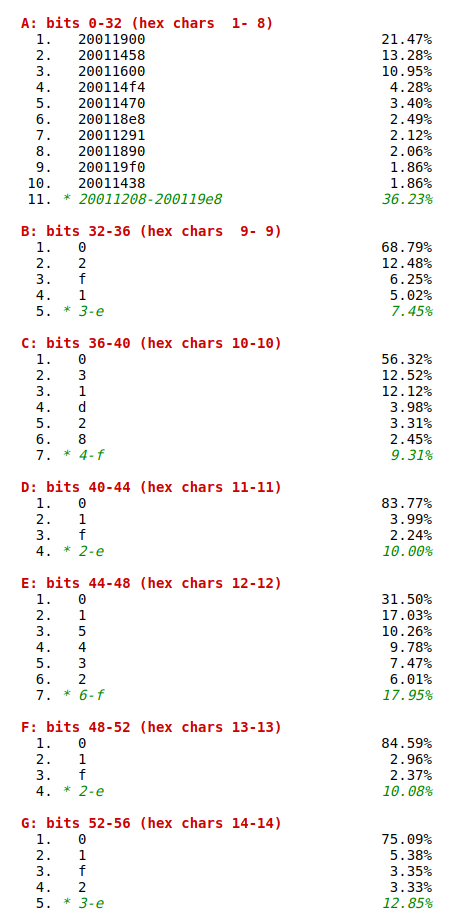
\includegraphics[width=0.3\textwidth]{dbscan}
\caption{DBSCAN}
\label{fig:dbscan}
\end{figure}

\section{贝叶斯网络}

将 IPv6 地址表示为随机向量, 我们可以很容易应用常见的统计模型. 我们选择使用贝叶斯网络来对 IPv6 地址段进行关联性分析.

贝叶斯网络是一种以有向无环图的形式表示联合分布随机变量的统计模型, 每个顶点代表一个变量, 从顶点 X 到顶点 Y 的一条边表示 Y 在统计上依赖于 X. 贝叶斯网络可以用来模拟包含许多变量的复杂对象, 将其分割为相互关联的小对象.

我们使用 BNFinder 程序构建 IPv6 地址的贝叶斯网络. 为了降低复杂度, 我们对网络进行约束: 每段只能依赖其之前的段. 我们将 IPv6 地址重新编码并于依赖性约束一起传递给 BNFinder 程序, BNFinder 程序运行后得到一个 cpd 文件, 其中存储了段间的关联性及具体的概率. 基于该文件, 我们可以依概率生成 IPv6 地址.

图~\ref{fig:bayes}~展示了样本集的贝叶斯网络.

\begin{figure}[htbp]
\centering
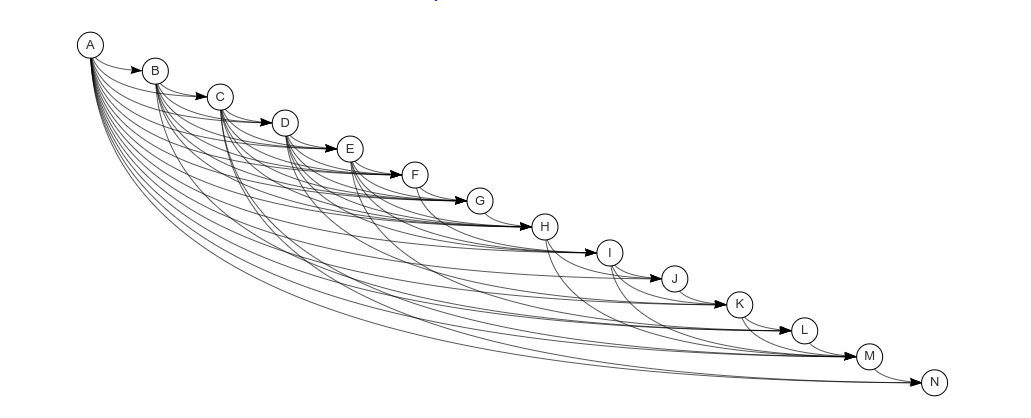
\includegraphics[width=0.6\textwidth]{bayes}
\caption{贝叶斯网络}
\label{fig:bayes}
\end{figure}

\chapter{模型评价}
\label{cha:evaluation}

我们尝试用 $2^{16}$ 个真实的 IPv6 地址训练贝叶斯网络模型, 然后利用该模型生成 256 个候选 IPv6 地址进行扫描, 并对扫描结果进行评估.

图~\ref{fig:generate}~显示了部分生成的 IPv6 地址. 图~\ref{fig:scan}~显示了使用 nmap 程序扫描生成的地址的结果.

\begin{figure}[htbp]
\centering
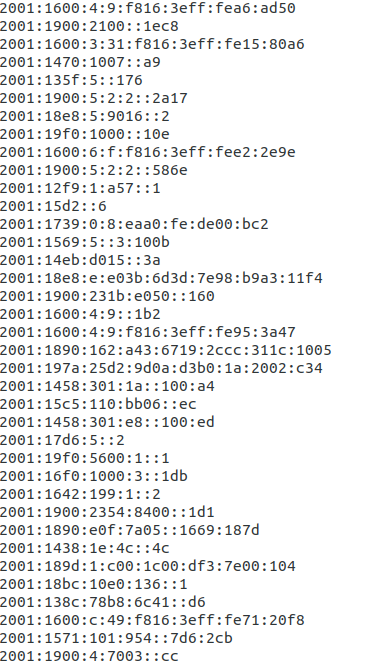
\includegraphics[width=0.3\textwidth]{generate}
\caption{地址生成}
\label{fig:generate}
\end{figure}

\begin{figure}[htbp]
\centering
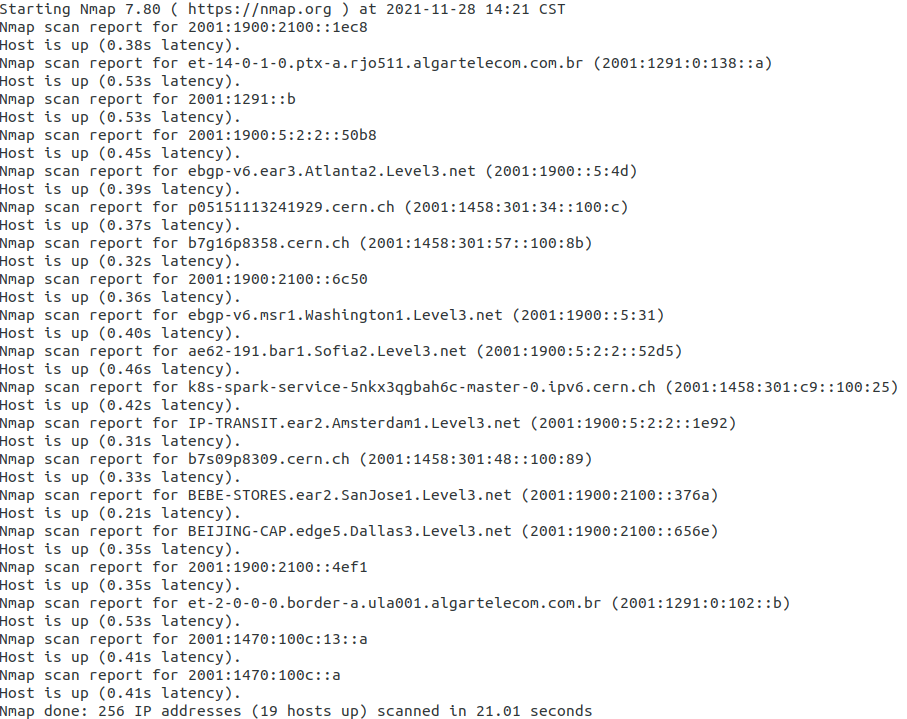
\includegraphics[width=0.5\textwidth]{scan}
\caption{地址扫描}
\label{fig:scan}
\end{figure}

生成的地址中约 7\% 是存活的, 该结果表明本文提出的基于贝叶斯网络的 IPv6 地址生成模型是一个卓有成效的 IPv6 网络扫描方法.

\chapter{结论}
\label{cha:conclusion}

为解决 IPv6 地址扫描问题, 本文提出了一种 IPv6 地址生成模型. 该模型尝试学习 IPv6 地址空间的结构特征, 基于 IPv6 地址每半字节的信息熵进行分段, 使用 DBSCAN 算法对每段进行聚类, 最后建立贝叶斯网络, 通过贝叶斯网络生成 IPv6 地址. 该模型将原本巨大到不可扫描的地址空间缩小到可扫描的大小, 有效提高了 IPv6 网络扫描的效率.


% 参考文献、致谢、附录等
\backmatter

% \bibliographystyle{gbt7714-unsrt.bst}%符合国标 GB/T 7714-2015 的文献风格
\bibliographystyle{zzubib.bst}%学校规范中示例文献风格
% \bibliography{ref/refs}%参考文献
\begin{thebibliography}{10}
\bibitem{ref:strayer}W. T. Strayer, C. E. Jones, F. Tchakountio, and R. R. Hain. SPIE-IPv6: Single IPv6 Packet Traceback. In Local Computer Networks, 2004. 29th Annual IEEE International Conference on, pages 118–125. IEEE, 2004.
\bibitem{ref:malone}D. Malone. Observations of IPv6 Addresses. In Passive and Active Network Measurement, 9th International Conference, PAM 2008, Cleveland, OH, USA, April 29-30, 2008. Proceedings, pages 21–30, 2008.
\bibitem{ref:gont}F. Gont and T. Chown. Network Reconnaissance in IPv6 Networks. RFC 7707, 2016.
\bibitem{ref:plonka}D. Plonka and A. Berger. Temporal and Spatial Classification of Active IPv6 Addresses. In Proceedings of the 2015 ACM Conference on Internet Measurement Conference, pages 509–522. ACM, 2015.
\end{thebibliography}

% 附录
% 研究生论文:综述
% \makeatletter
% \ifzzu@bachelor\else
%   \include{data/review}
% \fi
% \makeatother

% \makeatletter%致谢,研究生论文中在参考文献后,附录前
% \ifzzu@bachelor\else
%   \include{data/ack}
% \fi
% \makeatother

% % 附录
% % 本科生论文三个附录,分别是附表,外文翻译和外文原文
% % 研究生论文无具体要求
% \makeatletter
% \ifzzu@bachelor
%   \begin{appendix}
%     \input{data/app01}
%     \input{data/app02}
%     \input{data/app03}
%   \end{appendix}
% \fi
% \makeatother

% \makeatletter%个人简历
% \ifzzu@bachelor\else
%   \include{data/resume}%本科论文无要求
% \fi
% \makeatother

% \makeatletter%致谢,本科论文在最后
% \ifzzu@bachelor
%   \include{data/ack}
% \else\fi
% \makeatother

\end{document}
